\section{Testy jednostkowe - raport}

W celu zweryfikowania poprawności działania pojedynczych elementów programu takich jak metody klas i obiekty została wykorzystana metoda testowania tworzonego oprogramowania poprzez wykonywanie testów jednostkowych \textit{(ang. unit tests).}\newline
Do pliku rozwiązania w środowisku Visual Studio został dodany projekt, który składa się z klas odpowiednio testujących poszczególne klasy głównego projektu oprogramowania. Drzewo tego projektu przedstawiono na poniższym rysunku \ref{drzewo}.

\begin{figure}[ht!]
\centering
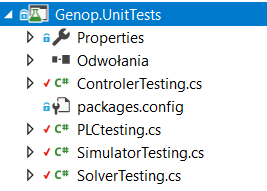
\includegraphics[scale=0.8]{listatest}
\caption{Drzewo projektu oprogramowania testów jednostkowych}
\label{drzewo}
\end{figure} 

Poniżej przedstawiono listing przykładowej klasy wykonującej testy jednostkowe metod występujących w klasie impelemtującej obiekt sterownika PLC. \newline

\begin{lstlisting}[language=C++]
namespace Genop.UnitTests
{
     /**
     * Klasa wykonujaca testy jednostkowe
     * niektorych z metod wystepujacych w
     * klasie PLC.
     */
    [TestClass]
    public class PLCTests
    {
        /**
         * Metoda testujaca metode
         * AutoIdentyfication(), kalkulujaca dane
         * i zwracajaca wartosc liczbowa
         */
        [TestMethod]
        public void AutoIdentyfication_Calculating_GetingValue()
        {
            // Arrange
            PLC plc1 = new PLC();

            // Act
            var resoult = plc1.AutoIdentyfication();

            // Assert
            Assert.IsNotNull(resoult);
        }
    }
}
\end{lstlisting}

Klasa oznaczona jako [TestClass] wskazuje na to, że zajmuje się ona testami. Podobnie oznaczenie metody [TestMethod] mówi o tym, że dana metoda jest testem. Test przeprowadza się zgodnie z konwencją AAA, czyli Arrange, Act and Assert. W miejscu Arrange, program zajmuje się stworzeniem zmiennych pomocniczych oraz testowanych obiektów, Act oznacza wykonanie wymaganych czynności testujących, natomiast na końcu wykonywana jest sekcja Assert - czyli porównanie wyników z wymaganiami danej metody. \newline

Na poniższym rysunku \ref{pozytyw} podano przykład metody, która pozytywnie przeszła test jednostkowy. Zwrócona przez nią wartość była, zgodnie z założeniami, wartością nie pustą.

\begin{figure}[ht!]
\centering
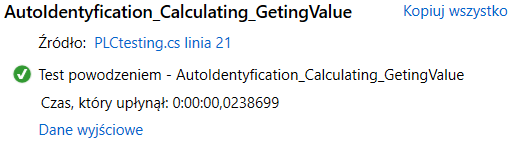
\includegraphics[scale=0.7]{testpozytyw}
\caption{Pozytywny wynik przeprowadzonego testu jednostkowego}
\label{pozytyw}
\end{figure} 

Na poniższym rysunku \ref{negatyw} podano przykład metody, która nie przeszła testu jednostkowego. Zwrócona przez nią wartość była nie zgodna z założeniami wartością pustą.


\begin{figure}[ht!]
\centering
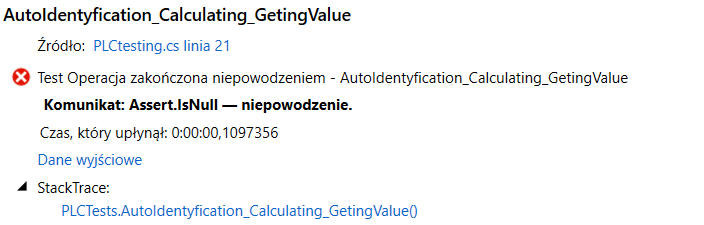
\includegraphics[scale=0.69]{testnegatyw}
\caption{Negatywny wynik przeprowadzonego testu jednostkowego}
\label{negatyw}
\end{figure} 